\documentclass[12pt]{cours}

\title{\textbf{\textsc{Diagramme des classes}}}
\author{Delay Emmanuel -- Desforêts Nicolas}


\usepackage{pgf-umlcd}



\begin{document}

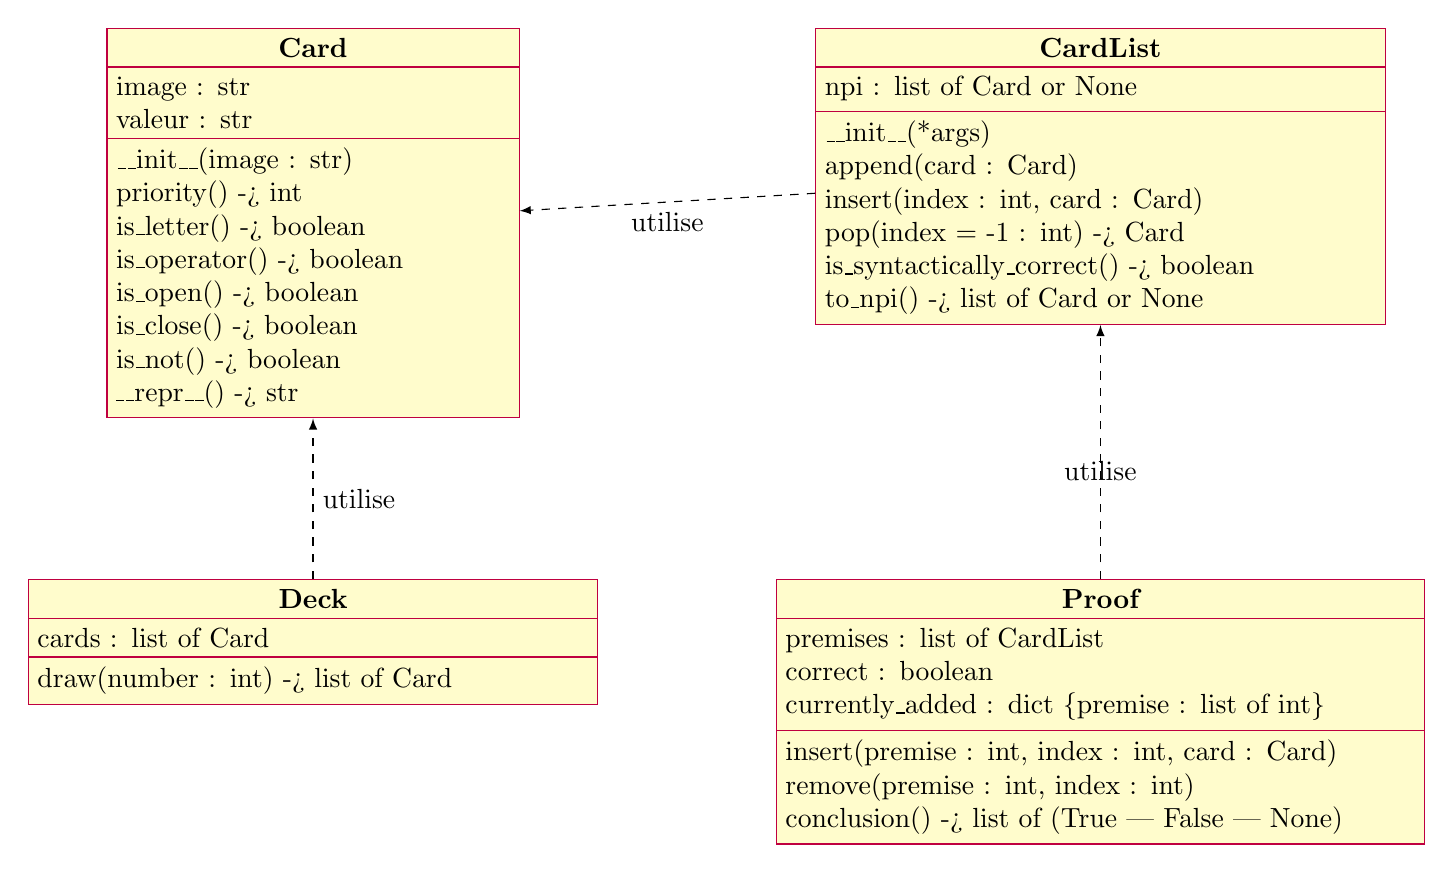
\begin{tikzpicture}
\begin{class}{Card}{0, 0}
\attribute{image : str}
\attribute{valeur : str}
\operation{\_\_init\_\_(image : str)}
\operation{priority() -> int}
\operation{is\_letter() -> boolean}
\operation{is\_operator() -> boolean}
\operation{is\_open() -> boolean}
\operation{is\_close() -> boolean}
\operation{is\_not() -> boolean}
\operation{\_\_repr\_\_() -> str}
\end{class}

\begin{class}[text width=7cm]{CardList}{10,0}
\attribute{npi : list of Card or None}
\operation{\_\_init\_\_(*args)}
\operation{append(card : Card)}
\operation{insert(index : int, card : Card)}
\operation{pop(index = -1 : int) -> Card}
\operation{is\_syntactically\_correct() -> boolean}
\operation{to\_npi() -> list of Card or None}
\end{class}

\draw[dashed,-latex] ({CardList}) -- node[below, midway]{utilise} (Card);

\begin{class}[text width=8cm]{Proof}{10, -7}
\attribute{premises : list of CardList}
\attribute{correct : boolean}
\attribute{currently\_added : dict \{premise : list of int\}}
\operation{insert(premise : int, index : int, card : Card)}
\operation{remove(premise : int, index : int)}
\operation{conclusion() -> list of (True | False | None)}
\end{class}

\draw[dashed,-latex] (Proof) --node[below, midway]{utilise} ({CardList});

\begin{class}[text width=7cm]{Deck}{0,-7}
\attribute{cards : list of Card}
\operation{draw(number : int) -> list of Card}
\end{class}

\draw[dashed,-latex] (Deck) --node[right, midway]{utilise} (Card);

\end{tikzpicture}


\end{document}

